\documentclass[a4paper]{article}

\usepackage[utf8]{inputenc}
\usepackage[english]{babel}
\usepackage{hyperref}
\usepackage{graphicx}
\usepackage{amsmath,amssymb,amsthm}
\usepackage{siunitx}
\usepackage{xcolor}
\usepackage{multicol}
\usepackage{caption}
\usepackage{appendix}
\usepackage{pdfpages}
\usepackage{fixltx2e}
\usepackage[version=4]{mhchem}
\usepackage{url}

\date{\today}
\author{Thomas Brzeski \and  Victor Dejans}
\title{Kinematic and Dynamic Analysis of a Linkage\\ Walschaerts Valve Gear}


\begin{document}

\maketitle

\section*{Introduction}

In the context of the subject \textit{Beweging en trillingen (H01N0A)} this report treats the analysis of the linkage in a Walschaerts valve gear (as seen in figure~\ref{fig:basistekening}), a system that is used in steam locomotives.

In a first section we define all links and joints with their geometric properties in the way we used them for the assignment. We also make the motion analysis of the linkage.

Second is the kinematic analysis which finds the positions, velocities and accelerations of each bar.

The final section reports upon the inverse dynamic analysis which finds the forces and torques on the linkages' joints when a driving torque is applied to the train's wheel.

\begin{figure}[h]
	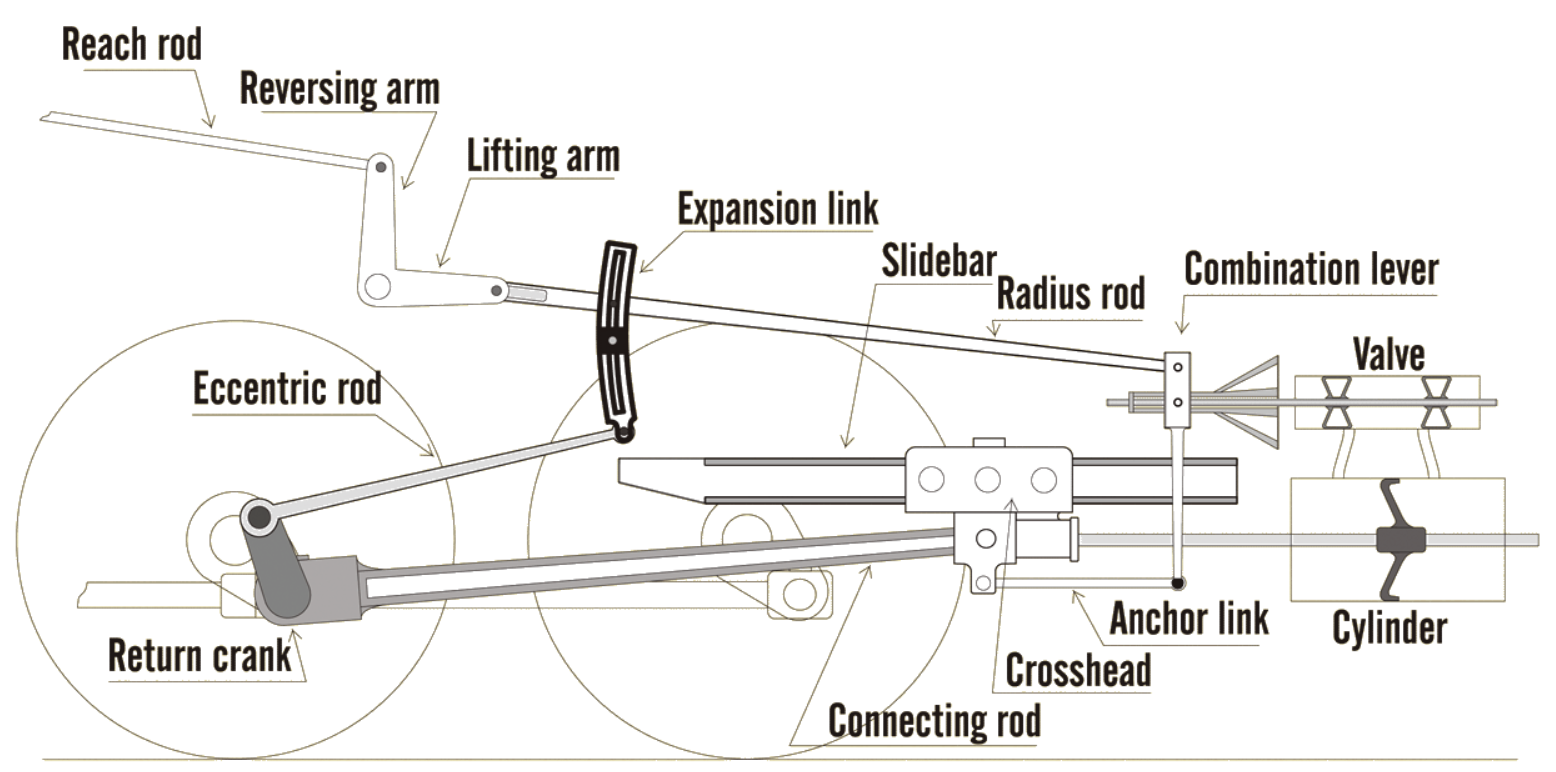
\includegraphics[width=0.7\textwidth]{wvgverslag.png}
	\centering
	\caption{Example of a Walschaerts valve gear. \cite{ove06}}
	\label{fig:basistekening}
\end{figure}

\newpage
\tableofcontents

\section{Definition of the mechanism}

\subsection{Schematic of the mechanism and definition of the parameters}

Walschaerts valve gear is a linkage that was used in steam locomotives. It connects the steam pistons and the train's wheels in a way that also regulates the steam flow.

Although in real life the pistons are the driving bodies and the wheels is the driven bodies, the assistants recommended us to analyse the mechanism in the opposite way. In this assignment, the driving torque is thus applied to the wheel instead of the pistons.

\subsection{Motion analysis}

The Walschaerts valve gear is a 12 bar linkage system with 16 joints. This makes the mobility \(M=3*(12-1)-16*2=1\).

\section{Kinematic analysis}

\subsection{Loop closure equations}

\subsection{Position analysis}

\subsection{Velocity analysis}

\subsection{Acceleration analysis}

\subsection{Checking of results}

\section{Dynamic analysis}

\subsection{Inverse dynamic analysis without gravity}

\subsection{Inverse dynamic analysis with gravity}

\subsection{Checking of results}

\bibliographystyle{unsrt}
\bibliography{walschaerts}


\end{document}